%\hspace*{0.82cm}\\[0.5cm]
\chapter{Software Requirements Specification}
\section{Introduction}
\subsection{Purpose}
\hspace*{0.82cm}This project aims at developing the Synchronization Manager for Android based devices.
Since there isn't any generic Synchronization Manger for android which works on all platforms
(Linux, Mac and Windows); this would help lots of people who work on two or more platforms. This
Synchronization Manager would be divided into two parts as server and client. The server would
reside on PC and client would be on Android Device. Client will gather information which is to be
synchronized.
\subsection{Document Conventions}
\hspace*{0.82cm}The following are the list of conventions and acronyms used in this document and the project as well,
privileges to the software:
\begin{itemize}
 \item \textbf{Client:} Intended users for the software.
 \item \textbf{SQL:} Structured Query Language; used to retrieve information from a database
 \item \textbf{SQL Server:} A server used to store data in an organized format
 \item \textbf{IEEE:} Institute of Electrical and Electronics Engineers
 \item \textbf{Layer:} Represents a section of the project
 \item \textbf{SYNC:} Synchronization
 \item \textbf{User Interface Layer:} The section of the assignment referring to what the user interacts with directly
 \item \textbf{Application Logic Layer:} The section of the assignment referring to the Web Server. This is where all 
computations are completed
 \item \textbf{Data Storage Layer:} The section of the assignment referring to where all data is recorded
 \item \textbf{Data flow diagram:} It shows the data flow between the entities
 \item \textbf{Use Case:} A broad level diagram of the project showing a basic overview
 \item \textbf{Boolean:} A true/false notation
 \item \textbf{Interface:} Something used to communicate across different mediums
\end{itemize}

\subsection{Intended Audience}
The intended audiences for this document are:
\begin{itemize}
 \item The team members of Innovative Android Synchronization Manager.
 \item The different Android users who are the clients.
\end{itemize}

This document will be reviewed frequently by the above audiences to check if the different
phases of the project are being completed by meeting the given requirements. If there are any changes
in the requirements in the course of the project they must be included in this document by making the
necessary changes.
\subsection{Product Scope}
\hspace*{0.82cm}The primary purpose of this is to have offline synchronization. At later stages this can be
extended to have online synchronization with services such as Ubuntu One for Linux. The software
can be made available as a paid service for corporations, users who want to backup their data.
\section{Overall Description}
\subsection{Product Perspective}
\hspace*{0.82cm}Since at the moment there does not exist any generic android client for synchronizing data
off-line, this product will simplify synchronizing data across multiple mobile device manufacturers.
This is a new self-contained product. It is basically for android users who would like to have a generic
client for off-line and on-line synchronization of their data. This data may include information like
contacts, calendar entries, messages, notes, audio, video files. It is particularly useful for the careful
user who prefers synchronizing data on their own servers rather than a third-party service provider.
Also, it will benefit users of android who are concerned about sending data on third-party servers.\\[0.5cm]
The following diagram represents the proposed architecture:

\begin{figure}[H]
  \centering
    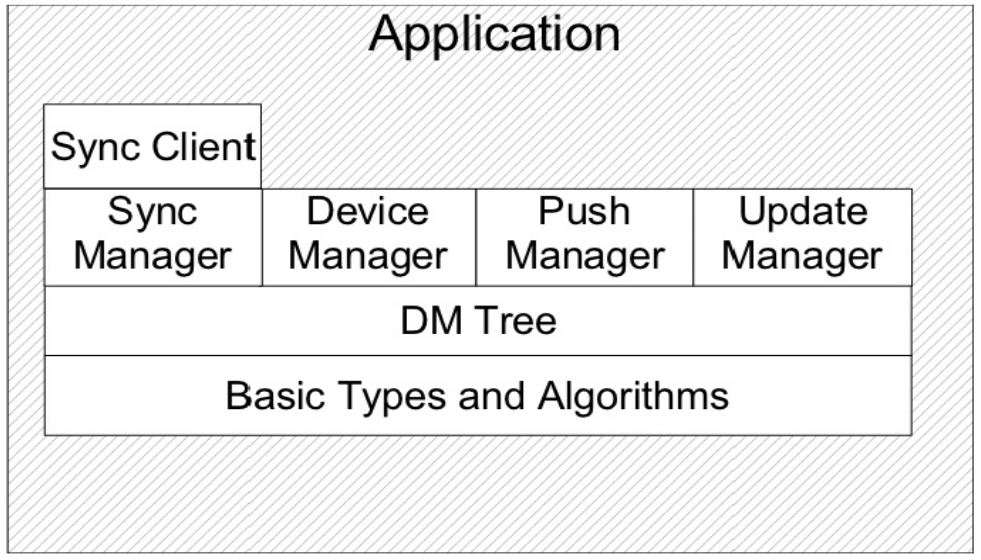
\includegraphics[scale=0.45]{project/images/client-architecture}
  \caption{\textbf{Architecture of Android Synchronization Manager (Client)}}
\end{figure}

\subsection{Product Functions}
\begin{itemize}
 \item Contact synchronization.
 \item Message synchronization.
 \item Calendar synchronization.
 \item Generating Reports.
 \item Managing logs of various activities in the phone (received/missed/dialed numbers).
 \item Backup of images, videos and other files.
\end{itemize}

\subsection{Operating Environment}
\begin{itemize}
 \item \textbf{For Client:} Android OS with v2.1 and above
 \item \textbf{For Server:} Any OS with Python 2.7, Qt 4.7+
\end{itemize}

\subsection{Design and Implementation Constraints}
\hspace*{0.82cm}This is a product primarily being developed for users of a specific mobile platform i.e.
Android. Hence users of mobile phones apart from android cannot use the features of this product.
Also it may be a challenge to create synchronization of data between an android device and a device
running on some other platform. Hence these constraints cannot be overlooked. Fortunately, this
product will be designed in a way that it will be extensible for integrating synchronization feature for
other platforms of mobile devices.\\[0.5cm]
\hspace*{0.82cm}But taking into consideration the huge number of mobile phone manufacturers, adding this
feature may take a considerable amount of time. These additions can be added keeping in view the
popularity of the platform this product is being ported into. Also, online synchronization might be
slower for additional authentication features like use of SSL and other security features.

\subsection{User Documentation}
\hspace*{0.82cm}User documentation would include the built-in help which will give a step by step guidance to
users of the software on how to effectively use this product. Apart from this, an online help system
through e-mails or mailing lists can also be set up. The product will be developed with out-most
importance being given to simplicity so that minimum developer intervention would be needed for
maintenance.

\subsection{Assumptions and Dependencies}
\hspace*{0.82cm}While developing this product it is being assumed that the android platform version used would
be v2.1 [and above]. The usage of the same on a lower version may give unexpected results. But the
product will be developed to keep it as cross-platform compatible as possible.

\section{External Interface Requirements}
\subsection{Hardware Interfaces}
\hspace*{0.82cm}Typical hardware interfaces that would be required would be the standard USB data cable
provided with the device. No other additional hardware interfacing would be needed to be bought by
the user. Also Bluetooth and/or Wi-Fi adapter on the server machine would be needed for
communication (in case USB cable is not available). Communication protocol would be developer
implemented and the user need not worry about communicating using this protocol. Hence this
product will be extremely user-friendly.

\subsection{Software Interfaces}
\hspace*{0.82cm}The product featured, requires a database to be maintained at both the ends - client and server.
Hence we will be deploying two different databases on both of them which will be in sync on
demand.\\[0.5cm]
\hspace*{0.82cm}The client DB will be implemented using SQLite and the server DB will be standard
PostgreSQL. The UI on client will be a typical android user interface using the default options
available at the time of development. UI on server will be implemented using Qt and python at the
backend.

\subsection{Communications Interfaces}
\hspace*{0.82cm}This product basically works on the client-server architecture. Hence a communication
mechanism between server and client has to be developed. This communication will be established
over https or local Bluetooth or Wi-Fi. USB cable is another option. E-mails can be used to
send/receive reports, log files.

\section{System Features}
\subsection{Synchronizing Contacts}
\hspace*{0.82cm}This feature is primarily why the product is being developed. This feature lets the user backup
contacts to the server. It will enable users to keep their server constantly updated with the newly
added contacts and their respective data.

\subsection{Synchronizing Messages}
\hspace*{0.82cm}This feature is basically used to backup SMSs and other drafts in the phone on to the server.
This feature is included as many users are keen on wanting to save all their conversations.

\subsection{Synchronizing files}
\hspace*{0.82cm}Along with all the data mentioned above, all the files on the user’s device can also be backed
up on the server. This will enable the user to store important information on the server and all the
information will be synchronized on a secure communication link.

\section{Other Non-functional Requirement}
\subsection{Security Requirements}
\hspace*{0.82cm}In our product, security is of out-most importance. Hence we need to implement
communication over HTTPS. For that it is required that the user should be in an environment where
the HTTPS port is not blocked. In case these ports are not enabled, an http connection will have to be
used. This means using http instead of https would lead to vulnerability of the user’s data to be sniffed
by third-party. Hence this should be considered as a security requirement of the product.